% Standalone build of every TikZ figure, one per page, at print size and in the paper's fonts
% (Times, Helvetica, Courier as IEEEtran sets them). Not part of the paper or the Overleaf zip:
% `make figures` compiles it and splits the pages into IMAGE/svg/*.svg and preview PNGs.
% The [OT1]{fontenc} line is a no-op under pdfLaTeX and makes XeTeX/Tectonic use Times too.
\documentclass[multi=odinfig, border=2pt]{standalone}
\usepackage[OT1]{fontenc}
\renewcommand{\rmdefault}{ptm}
\renewcommand{\sfdefault}{phv}
\renewcommand{\ttdefault}{pcr}
\usepackage{graphicx}
\usepackage{tikz}
\usetikzlibrary{positioning,fit,arrows.meta,shapes.geometric,backgrounds,calc,matrix}
% Shared TikZ styles for the Odin III paper figures (IMAGE/fig_*.tex).
% Needs: \usepackage{tikz} and
%   \usetikzlibrary{positioning,fit,arrows.meta,shapes.geometric,backgrounds,calc,matrix}
% loaded first (odin3.tex and IMAGE/figures.tex both do). Input this file once, in the preamble.
%
% Palette: the greens and browns of a tree and its greenery, with black for Odin's raven as the
% strong ink. Green = ColorBrewer "Greens", brown = a warm earth ramp. Text is dark on the light
% fills and white only on the dark browns and the black. Build status is coded twice, by fill and
% by border, so it survives a black-and-white print:
%   built        mid-green fill,  solid dark-green border
%   in progress  pale-green fill, solid green border
%   specified    white fill,      dashed green border
%   planned      white fill,      dotted brown border

% ---- colours ------------------------------------------------------------------------------
\definecolor{o3ink}{HTML}{111111}      % text and arrows: the raven's black
\definecolor{o3sub}{HTML}{4E342E}      % secondary text (sub-project tags, notes): dark brown
\definecolor{o3grn9}{HTML}{00441B}
\definecolor{o3grn8}{HTML}{006D2C}
\definecolor{o3grn7}{HTML}{238B45}
\definecolor{o3grn5}{HTML}{74C476}
\definecolor{o3grn4}{HTML}{A1D99B}
\definecolor{o3grn3}{HTML}{C7E9C0}
\definecolor{o3grn2}{HTML}{E5F5E0}
\definecolor{o3grn1}{HTML}{F7FCF5}
\definecolor{o3brn9}{HTML}{3E2723}     % root system, dark brown (white text only)
\definecolor{o3brn8}{HTML}{5D4037}
\definecolor{o3brn7}{HTML}{4E342E}
\definecolor{o3brn6}{HTML}{6D4C41}     % trunk
\definecolor{o3brn5}{HTML}{8D6E63}
\definecolor{o3brn4}{HTML}{C9B6A4}     % branches, lighter brown
\definecolor{o3brn3}{HTML}{E0D3C6}
\definecolor{o3brn2}{HTML}{F1E9DF}
\definecolor{o3brn1}{HTML}{F8F4EE}

% ---- text helpers -------------------------------------------------------------------------
% A second, smaller line in a node: \odinsub{2C}.
\newcommand{\odinsub}[1]{{\scriptsize\color{o3sub}#1}}
% Code names inside figures (the paper's \code is not defined in the standalone build).
\newcommand{\odintt}[1]{\texttt{#1}}

% Scale a figure down only if it is wider than #1 (it never scales up). Each figure is drawn
% at its print size, so this is a safety net; a scaled figure writes "ODINFIT" to the log.
\newsavebox{\odinfigbox}
\newcommand{\odinfit}[2]{%
  \sbox{\odinfigbox}{\ignorespaces#2\unskip}%
  \ifdim\wd\odinfigbox>#1\relax
    \typeout{ODINFIT: figure scaled from \the\wd\odinfigbox\space to \the#1}%
    \resizebox{#1}{!}{\usebox{\odinfigbox}}%
  \else
    \usebox{\odinfigbox}%
  \fi}

% ---- TikZ styles --------------------------------------------------------------------------
\tikzset{
  % every figure
  odin/.style={font=\footnotesize, color=o3ink, line join=round,
               >={Stealth[length=3.4pt, width=2.8pt]},
               % node text breaks the same way in any class: no hyphens, loose lines rather than overfull
               execute at begin node={\hyphenpenalty=10000\exhyphenpenalty=10000%
                 \tolerance=9999\emergencystretch=10pt}},
  % shapes
  box/.style={draw, rectangle, rounded corners=1.6pt, align=center, line width=0.55pt,
              inner xsep=2.5pt, inner ysep=2pt, minimum height=6.5mm},
  store/.style={draw, cylinder, shape border rotate=90, aspect=0.16, align=center,
                line width=0.55pt, inner xsep=2pt, inner ysep=1pt, minimum height=8mm},
  plain/.style={align=center, inner sep=1pt},
  % build status (combine with a shape: [box, built])
  built/.style={fill=o3grn4, draw=o3grn8, solid},
  inprog/.style={fill=o3grn2, draw=o3grn7, solid},
  spec/.style={fill=white, draw=o3grn7, dash pattern=on 2.4pt off 1.4pt},
  planned/.style={fill=white, draw=o3brn5, dash pattern=on 0.6pt off 1.3pt,
                  line width=0.75pt},
  % neutral fills for structure figures
  neutral/.style={fill=o3brn2, draw=o3brn6, solid},
  light/.style={fill=o3grn1, draw=o3grn7, solid},
  external/.style={fill=o3brn2, draw=o3brn6, dash pattern=on 3pt off 1.2pt on 0.6pt off 1.2pt},
  emph/.style={line width=1.3pt},
  % grouped regions, drawn on the background layer
  region/.style={draw=o3brn4, fill=o3brn1, rounded corners=3pt, line width=0.5pt,
                 inner sep=4pt},
  bluregion/.style={draw=o3grn3, fill=o3grn1, rounded corners=3pt, line width=0.5pt,
                    inner sep=4pt},
  regionlabel/.style={font=\scriptsize\bfseries, color=o3brn7, inner sep=1.5pt},
  % arrows
  flow/.style={->, line width=0.55pt, draw=o3ink},
  flowplanned/.style={->, line width=0.6pt, draw=o3brn6, dash pattern=on 0.6pt off 1.3pt},
  ref/.style={->, line width=0.5pt, draw=o3grn8, dash pattern=on 2.4pt off 1.4pt},
  edgelabel/.style={font=\scriptsize, color=o3sub, inner sep=1pt, fill=white},
  % records: a header row and field rows, built with \matrix (see fig_ir_model.tex)
  record/.style={matrix of nodes, ampersand replacement=\&, row sep=-\pgflinewidth,
                 inner sep=0pt, nodes={draw=o3brn6, line width=0.5pt, fill=white,
                 font=\scriptsize, anchor=center, align=left, inner xsep=2.5pt,
                 inner ysep=1.2pt, minimum height=4.4mm}},
  rechead/.style={fill=o3grn3, font=\scriptsize\bfseries, align=center},
  % legend keys
  legendkey/.style={box, minimum width=4.2mm, minimum height=2.6mm, inner sep=0pt},
  legendtext/.style={font=\scriptsize, inner sep=1pt, text height=1.5ex, text depth=0.3ex},
}

% \odinlegend{<node options, e.g. anchor=north east, at={(x,y)}>}
% The build-status key, one row, as a single node so figures can place it like any node.
\newcommand{\odinlegend}[1]{%
  \matrix[ampersand replacement=\&, column sep=1.2pt, inner sep=2pt, draw=o3brn4,
          rounded corners=2pt, fill=white, line width=0.4pt, #1]{%
    \node[legendkey, built]{};   \& \node[legendtext]{built};       \& \node{\hspace{3pt}}; \&
    \node[legendkey, inprog]{};  \& \node[legendtext]{in progress}; \& \node{\hspace{3pt}}; \&
    \node[legendkey, spec]{};    \& \node[legendtext]{specified};   \& \node{\hspace{3pt}}; \&
    \node[legendkey, planned]{}; \& \node[legendtext]{planned};     \\
  };}

% \odinrecord{<name>}{<matrix options: position, nodes={text width=...}>}{<header>}{<rows>}
% A record (struct) as a one-column matrix: a header cell, then one cell per field, rows
% separated by \\ and ended by \\. Cells are <name>-<row>-1, so edges can leave from a field.
\newcommand{\odinrecord}[4]{%
  \matrix[record, #2] (#1) {|[rechead]| #3 \\ #4};}

\begin{document}
\begin{odinfig}% Odin III system pipeline (DESIGN.md sections 3, 4.0, 6, 9, 12; PHASE3.md), status 2026-10-11.
% Wide figure: \textwidth (figure*). Row 1 runs left to right (project input to word-level IR),
% row 2 right to left through the passes, row 3 holds the writers and the build-status key.
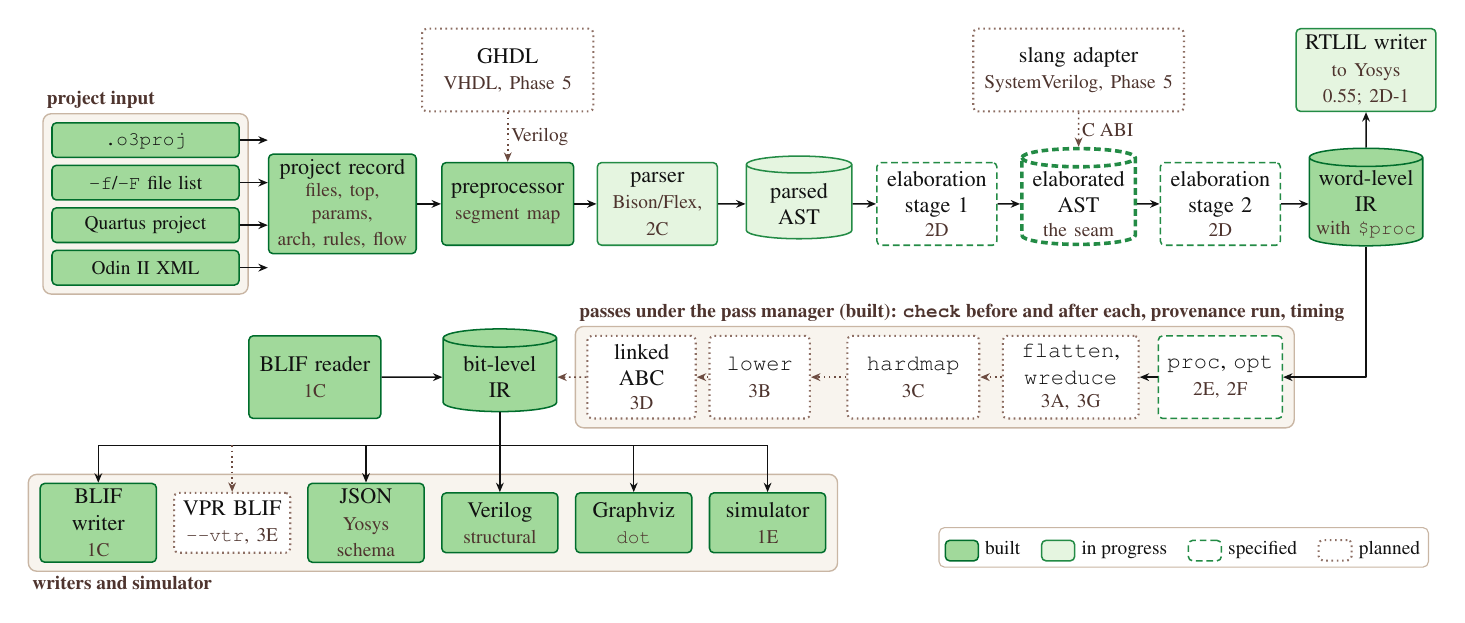
\begin{tikzpicture}[odin, node distance=3mm,
  box/.append style={minimum height=10.5mm}, store/.append style={minimum height=10.5mm}]
  % ---- row 1: project input and the Verilog front end ----------------------------------
  \begin{scope}[every node/.append style={box, built, font=\scriptsize,
                text width=22mm, minimum height=4.4mm, inner ysep=1pt}]
    \node (o3proj) at (1.45, 0.81)  {\odintt{.o3proj}};
    \node (flist)  at (1.45, 0.27)  {\odintt{-f}/\odintt{-F} file list};
    \node (qsf)    at (1.45, -0.27) {Quartus project};
    \node (odin2)  at (1.45, -0.81) {Odin~II XML};
  \end{scope}
  \node[box, built, text width=17mm] (record) at (3.95, 0)
       {project record\\\odinsub{files, top, params,\\arch, rules, flow}};
  \node[box, built, text width=15mm] (pp) at (6.05, 0) {preprocessor\\\odinsub{segment map}};
  \node[box, inprog, text width=13.5mm] (parser) at (7.95, 0) {parser\\\odinsub{Bison/Flex, 2C}};
  \node[store, inprog, text width=12mm] (past) at (9.75, 0) {parsed\\AST};
  \node[box, spec, text width=13.5mm] (st1) at (11.5, 0) {elaboration\\stage 1\\[-1pt]\odinsub{2D}};
  \node[store, spec, emph, text width=13mm] (east) at (13.3, 0) {elaborated\\AST\\[-1pt]\odinsub{the seam}};
  \node[box, spec, text width=13.5mm] (st2) at (15.1, 0) {elaboration\\stage 2\\[-1pt]\odinsub{2D}};
  \node[store, built, text width=13mm] (wir) at (16.95, 0)
       {word-level\\IR\\[-1pt]\odinsub{with \odintt{\$proc}}};

  % ---- row 0: other front ends and the Yosys bridge -----------------------------------
  \node[box, planned, text width=20mm] (ghdl) at (6.05, 1.7)
       {GHDL\\\odinsub{VHDL, Phase 5}};
  \node[box, planned, text width=25mm] (slang) at (13.3, 1.7)
       {slang adapter\\\odinsub{SystemVerilog, Phase 5}};
  \node[box, inprog, text width=16mm] (rtlil) at (16.95, 1.7)
       {RTLIL writer\\\odinsub{to Yosys 0.55; 2D-1}};

  % ---- row 2: passes (right to left) ----------------------------------------------------
  \node[box, spec, text width=14mm] (procopt) at (15.1, -2.2) {\odintt{proc}, \odintt{opt}\\\odinsub{2E, 2F}};
  \node[box, planned, text width=15.5mm] (flat) at (13.2, -2.2)
       {\odintt{flatten},\\\odintt{wreduce}\\[-1pt]\odinsub{3A, 3G}};
  \node[box, planned, text width=15mm] (hmap) at (11.2, -2.2) {\odintt{hardmap}\\\odinsub{3C}};
  \node[box, planned, text width=11mm] (lower) at (9.25, -2.2) {\odintt{lower}\\\odinsub{3B}};
  \node[box, planned, text width=12mm] (abc) at (7.75, -2.2) {linked\\ABC\\[-1pt]\odinsub{3D}};
  \node[store, built, text width=13mm] (bir) at (5.95, -2.2) {bit-level\\IR};
  \node[box, built, text width=15mm] (rblif) at (3.6, -2.2) {BLIF reader\\\odinsub{1C}};

  % ---- row 3: writers and the simulator -------------------------------------------------
  \begin{scope}[every node/.append style={box, text width=13mm, minimum height=7.6mm}]
    \node[built]   (wblif) at (0.85, -4.05) {BLIF writer\\\odinsub{1C}};
    \node[planned] (wvtr)  at (2.55, -4.05) {VPR BLIF\\\odinsub{\odintt{--vtr}, 3E}};
    \node[built]   (wjson) at (4.25, -4.05) {JSON\\\odinsub{Yosys schema}};
    \node[built]   (wver)  at (5.95, -4.05) {Verilog\\\odinsub{structural}};
    \node[built]   (wdot)  at (7.65, -4.05) {Graphviz\\\odinsub{\odintt{dot}}};
    \node[built]   (sim)   at (9.35, -4.05) {simulator\\\odinsub{1E}};
  \end{scope}

  % ---- edges ----------------------------------------------------------------------------
  \foreach \n in {o3proj, flist, qsf, odin2}
    \draw[flow] (\n.east) -- (\n.east -| record.west);
  \draw[flow] (record) -- (pp);
  \draw[flow] (pp) -- (parser);
  \draw[flow] (parser) -- (past);
  \draw[flow] (past) -- (st1);
  \draw[flow] (st1) -- (east);
  \draw[flow] (east) -- (st2);
  \draw[flow] (st2) -- (wir);
  \draw[flowplanned] (ghdl) -- node[edgelabel, right, fill=none] {Verilog} (pp);
  \draw[flowplanned] (slang) -- node[edgelabel, right, fill=none] {C ABI} (east);
  \draw[flow] (wir) -- (rtlil);
  \draw[flow] (wir.south) |- (procopt.east);
  \draw[flow] (procopt) -- (flat);
  \draw[flowplanned] (flat) -- (hmap);
  \draw[flowplanned] (hmap) -- (lower);
  \draw[flowplanned] (lower) -- (abc);
  \draw[flowplanned] (abc) -- (bir);
  \draw[flow] (rblif) -- (bir);
  % bus from the bit-level IR to the writers
  \coordinate (rail) at ($(bir.south)+(0,-0.42)$);
  \draw[line width=0.55pt, draw=o3ink] (bir.south) -- (rail);
  \draw[line width=0.55pt, draw=o3ink] (rail -| wblif) -- (rail -| sim);
  \foreach \n in {wblif, wjson, wver, wdot, sim}
    \draw[flow] (rail -| \n) -- (\n.north);
  \draw[flowplanned] (rail -| wvtr) -- (wvtr.north);

  % ---- regions (background) -------------------------------------------------------------
  \begin{scope}[on background layer]
    \node[region, fit=(o3proj)(odin2), inner xsep=3pt, inner ysep=3pt,
          label={[regionlabel, anchor=south west]north west:project input}] (rin) {};
    \node[region, fit=(procopt)(abc), inner ysep=3pt,
          label={[regionlabel, anchor=south west]north west:{passes under the pass manager
          (built): \odintt{check} before and after each, provenance run, timing}}]
          (rpm) {};
    \node[region, fit=(wblif)(sim), inner ysep=3pt,
          label={[regionlabel, anchor=north west]south west:writers and simulator}] (rout) {};
  \end{scope}

  \odinlegend{anchor=south east, at={(17.75, -4.62)}}
\end{tikzpicture}
\end{odinfig}
\begin{odinfig}% Project input (DESIGN.md section 4.0, 2B spec PRJ-1..PRJ-18): every format fills one
% design-owned project record; read_verilog, the tech library, dump_project and (Phase 4) the
% partial mapper only read it. Single column: \columnwidth.
\begin{tikzpicture}[odin,
  fmt/.style={box, built, text width=18mm, minimum height=10.5mm},
  use/.style={box, text width=18.4mm, minimum height=11mm, inner xsep=1.5pt},
  fld/.style={draw=o3grey6, fill=white, line width=0.5pt, font=\scriptsize, align=left,
              text width=40mm, minimum height=5.6mm, inner xsep=2.2pt, inner ysep=1pt},
  fldh/.style={fld, fill=o3blue4, draw=o3blue8, font=\footnotesize, align=center,
               text width=80mm+3.9pt, minimum height=5mm}]
  % ---- the four formats --------------------------------------------------------------------
  \foreach \n/\x/\t/\s in {
      o3/1.05/\odintt{.o3proj}/{native; arch,\\rules and flow},
      fl/3.25/file list/{EDA style:\\\odintt{-f}, \odintt{-F}},
      qs/5.45/Quartus/{\odintt{.qpf}, \odintt{.qsf},\\\odintt{.qip}},
      ox/7.65/Odin~II XML/{the \odintt{config}\\file}}
    \node[fmt] (\n) at (\x, 0) {\t\\\odinsub{\s}};

  % ---- the record: a header and two columns of fields ---------------------------------------
  \node[fldh] (rh) at (4.35, -1.45) {project record \odinsub{(design-owned; 2B)}};
  \node[fld, anchor=north west] (f1) at ($(rh.south west)+(0,\pgflinewidth)$)
       {files: path as given and resolved, location, language, library};
  \node[fld, anchor=north west] (f3) at ($(f1.south west)+(0,\pgflinewidth)$)
       {top and its location; params \odintt{scope.name = value}};
  \node[fld, anchor=north west] (f5) at ($(f3.south west)+(0,\pgflinewidth)$)
       {mapping rules: \odintt{map}, \odintt{split}, \odintt{limit}, patterns (stored)};
  \node[fld, anchor=north west] (f7) at ($(f5.south west)+(0,\pgflinewidth)$)
       {flow script; ignored keys; duplicates};
  \node[fld, anchor=north west] (f2) at ($(f1.north east)+(-\pgflinewidth,0)$)
       {library files and directories, \odintt{libext}, include directories, defines};
  \node[fld, anchor=north west] (f4) at ($(f2.south west)+(0,\pgflinewidth)$)
       {architecture: \odintt{.o3lib}, VPR XML or device};
  \node[fld, anchor=north west] (f6) at ($(f4.south west)+(0,\pgflinewidth)$)
       {inventory (\odintt{available}); overrides (\odintt{hide}, \odintt{cell from})};
  \node[fld, anchor=north west] (f8) at ($(f6.south west)+(0,\pgflinewidth)$)
       {revision; output (Odin~II XML)};
  \node[fit=(rh)(f1)(f8), inner sep=0pt, draw=o3blue8, line width=0.7pt] (rec) {};

  % ---- the readers of the record ------------------------------------------------------------
  \node[use, inprog]  (rv) at (1.05, -5.0) {{\scriptsize\odintt{read\_verilog}}\\\odinsub{preprocess, parse,\\[-2pt]elaborate}};
  \node[use, built]   (rt) at (3.25, -5.0) {{\scriptsize\odintt{read\_techlib}}\\\odinsub{\odintt{.o3lib}, 1G}};
  \node[use, planned] (pm) at (5.45, -5.0) {{\scriptsize\odintt{partial\_map}}\\\odinsub{Phase 4}};
  \node[use, built]   (dp) at (7.65, -5.0) {{\scriptsize\odintt{dump\_project}}\\\odinsub{JSON: the corpus\\[-2pt]oracle record}};

  \foreach \n in {o3, fl, qs, ox} \draw[flow] (\n.south) -- (\n.south |- rec.north);
  \foreach \n in {rv, rt, dp}     \draw[flow] (\n.north |- rec.south) -- (\n.north);
  \draw[flowplanned] (pm.north |- rec.south) -- (pm.north);

  \odinlegend{anchor=north, at={(4.35, -5.75)}}
\end{tikzpicture}
\end{odinfig}
\begin{odinfig}% Two-stage elaboration with the elaborated AST as the seam (2D spec section 2, EL-2, EL-4).
% Stage 1 is Verilog-only; stage 2 is shared by every front end. The slang adapter (Phase 5)
% builds the elaborated form through the C ABI and enters at stage 2. Wide: \textwidth.
\begin{tikzpicture}[odin,
  stage/.style={box, text width=34mm, align=left, minimum height=21mm},
  list/.style={font=\scriptsize, align=left}]
  % ---- the main row ------------------------------------------------------------------------
  \node[box, neutral, text width=15mm, minimum height=12mm] (vf) at (0.95, 0)
       {Verilog-2005\\files\\[-1pt]\odinsub{preprocessed, 2B}};
  \node[store, built, text width=14mm, minimum height=14mm] (ps) at (2.95, 0)
       {parsed\\store\\[-1pt]\odinsub{form \odintt{PARSED}}\\[-2pt]\odinsub{2C}};
  \node[stage, inprog] (s1) at (5.84, 0)
       {\textbf{stage 1} (Verilog only)\\[1pt]
        \scriptsize module lookup, top selection\\
        \scriptsize \odintt{\#()}, \odintt{defparam}, project params\\
        \scriptsize specialisation\\
        \scriptsize \odintt{generate}\\
        \scriptsize constant functions\\
        \scriptsize implicit nets};
  \node[store, spec, emph, text width=30mm, inner xsep=4pt, inner ysep=0pt, minimum height=20mm] (es) at (9.81, 0)
       {\textbf{elaborated store}\\[-1pt]\odinsub{the seam, form}\\[-2pt]\odinsub{\odintt{ELABORATED}}\\[1pt]
        \scriptsize no \odintt{generate} or \odintt{defparam}\\
        \scriptsize constants resolved\\
        \scriptsize one \odintt{MODULE} per\\
        \scriptsize specialisation};
  \node[stage, spec] (s2) at (13.78, 0)
       {\textbf{stage 2} (every front end)\\[1pt]
        \scriptsize binding (symbol table)\\
        \scriptsize Yosys widths and signedness\\
        \scriptsize word cells, drivers, \odintt{\$mem}\\
        \scriptsize \odintt{always} $\rightarrow$ \odintt{\$proc} cells\\
        \scriptsize inlining, initial values};
  \node[store, built, text width=16mm, minimum height=14mm] (ir) at (16.94, 0)
       {word-level\\IR\\[-1pt]\odinsub{+ \odintt{\$proc} (2D-1)}};

  % ---- around the seam -----------------------------------------------------------------------
  \node[box, light, text width=40mm, align=center] (chk) at (9.81, 2.0)
       {\odintt{odin3\_ast\_check}, rule 7\\\odinsub{enforces the elaborated subset}};
  \node[box, planned, text width=36mm] (sl) at (9.81, -2.35)
       {slang adapter (C++)\\\odinsub{\odintt{odin3\_ast\_*} builders; Phase 5}};
  \node[box, built, text width=19.5mm] (rt) at (16.94, -2.35)
       {\odintt{write\_rtlil}\\\odinsub{2D-1}};
  \node[box, external, text width=28mm] (yo) at (13.6, -2.35)
       {Yosys 0.55 (Parmys's)\\\odinsub{equivalence oracle}};

  % ---- edges ---------------------------------------------------------------------------------
  \draw[flow] (vf) -- (ps);
  \draw[flow] (ps) -- (s1);
  \draw[flow] (s1) -- (es);
  \draw[flow] (es) -- (s2);
  \draw[flow] (s2) -- (ir);
  \draw[flow] (ir) -- (rt);
  \draw[flow] (rt) -- (yo);
  \draw[flowplanned] (sl) -- node[edgelabel, right] {\odintt{odin3\_ast\_elaborate} (C ABI)} (es);
  \draw[line width=0.5pt, draw=o3blue7, dash pattern=on 2.4pt off 1.4pt] (chk) -- (es);

  % ---- regions -------------------------------------------------------------------------------
  \begin{scope}[on background layer]
    \node[region, fit=(vf)(ps)(s1), inner sep=5pt,
          label={[regionlabel, anchor=south west]north west:stage 1: Verilog-specific}] {};
    \node[region, fit=(s2)(ir), inner sep=5pt,
          label={[regionlabel, anchor=south east]north east:stage 2: shared by every front end}] {};
  \end{scope}

  \odinlegend{anchor=west, at={(0.0, -2.35)}}
\end{tikzpicture}
\end{odinfig}
\begin{odinfig}% src/util containers (1A spec): the only generic containers in the tree, all built on one
% allocation wrapper whose test hook fails the n-th allocation. Arrows point from a container to
% what it uses. Single column: \columnwidth.
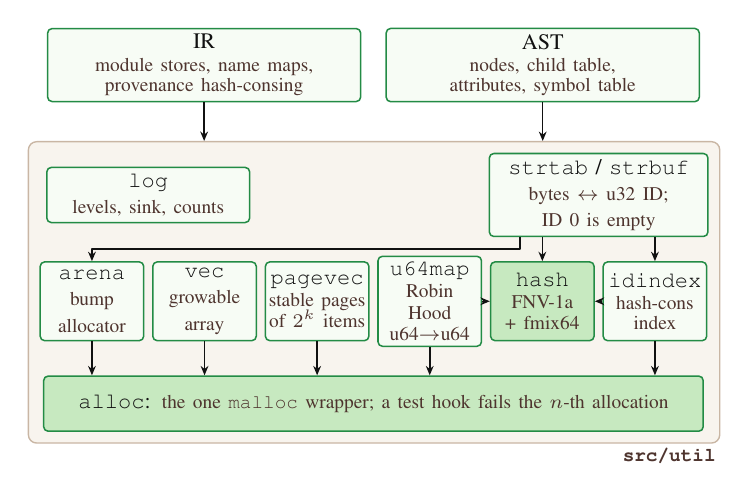
\begin{tikzpicture}[odin,
  c/.style={box, light, text width=12.3mm, minimum height=10mm, inner xsep=1.2pt},
  wide/.style={box, light, minimum height=7mm}]
  % ---- containers (tier 1) -----------------------------------------------------------------
  \node[c] (arena) at (0.667, 0) {\odintt{arena}\\\odinsub{bump allocator}};
  \node[c] (vec)   at (2.097, 0) {\odintt{vec}\\\odinsub{growable array}};
  \node[c] (pv)    at (3.527, 0) {\odintt{pagevec}\\\odinsub{stable pages\\[-2pt]of $2^k$ items}};
  \node[c] (u64)   at (4.957, 0) {\odintt{u64map}\\\odinsub{Robin Hood\\[-2pt]u64$\to$u64}};
  \node[c, fill=o3grn3] (hash) at (6.387, 0) {\odintt{hash}\\\odinsub{FNV-1a\\[-2pt]+ fmix64}};
  \node[c] (idx)   at (7.817, 0) {\odintt{idindex}\\\odinsub{hash-cons\\[-2pt]index}};
  % ---- foundation (tier 0) and strings / log (tier 2) ----------------------------------------
  \node[wide, fill=o3grn3, text width=82mm] (alloc) at (4.242, -1.3)
       {\odintt{alloc}: \odinsub{the one \odintt{malloc} wrapper; a test hook fails the $n$-th allocation}};
  \node[wide, text width=26mm] (str) at (7.102, 1.35)
       {\odintt{strtab} / \odintt{strbuf}\\\odinsub{bytes $\leftrightarrow$ u32 ID; ID 0 is empty}};
  \node[wide, text width=24mm] (log) at (1.382, 1.35) {\odintt{log}\\\odinsub{levels, sink, counts}};

  % ---- uses ----------------------------------------------------------------------------------
  \foreach \n in {arena, vec, pv, u64, idx} \draw[flow] (\n.south) -- (\n.south |- alloc.north);
  \draw[flow] (u64) -- (hash);
  \draw[flow] (idx) -- (hash);
  \draw[flow] (str.south -| hash) -- (hash.north);
  \draw[flow] (str.south -| idx) -- (idx.north);
  \coordinate (corr) at ($(str.south)!0.5!(str.south |- idx.north)$);
  \draw[flow] ($(str.south west)+(4mm,0)$) |- (corr -| arena) -- (arena.north);

  % ---- the users ---------------------------------------------------------------------------
  \begin{scope}[on background layer]
    \node[region, fit=(alloc)(arena)(idx)(str)(log), inner sep=4pt,
          label={[regionlabel, anchor=north east]south east:\odintt{src/util}}] (util) {};
  \end{scope}
  \node[box, light, text width=38mm] (ir) at (2.092, 3.0)
       {IR\\\odinsub{module stores, name maps,\\[-2pt]provenance hash-consing}};
  \node[box, light, text width=38mm] (ast) at (6.392, 3.0)
       {AST\\\odinsub{nodes, child table,\\[-2pt]attributes, symbol table}};
  \draw[flow] (ir.south) -- (ir.south |- util.north);
  \draw[flow] (ast.south) -- (ast.south |- util.north);
\end{tikzpicture}
\end{odinfig}
\begin{odinfig}% Odin III IR object model (docs/IR.md sections 1-6, src/ir/ir_internal.h). Record sizes are
% sizeof() on x86-64 (gcc 13): node 40 B, pin 24 B, net 40 B, wire 40 B. Wide: \textwidth.
% Solid arrows are typed 32-bit ID references; double-headed arrows are the two directions of
% one relation; grey arrows are ownership.
\begin{tikzpicture}[odin,
  idref/.style={flow, draw=o3blue8},
  idref2/.style={idref, <->},
  owns/.style={flow, draw=o3grey6},
  lab/.style={edgelabel, fill=none, inner sep=1pt}]
  % ---- design and module -------------------------------------------------------------------
  \odinrecord{design}{anchor=north, nodes={text width=26mm},
              row 1/.style={nodes={fill=o3blue4}}, at={(1.39, 0)}}{Design}{
    strings (names, paths) \\ provenance store \\ pass-run table \\ tombstones \\
    cell-type table \\ modules[\,] \\ top \\}
  \odinrecord{module}{anchor=north, nodes={text width=31mm},
              row 1/.style={nodes={fill=o3blue4}}, at={(4.92, 0)}}{Module (IR-18)}{
    nodes: \odintt{pagevec} of node \\ pins: \odintt{pagevec} of pin \\
    nets: \odintt{pagevec} of net \\ wires: \odintt{pagevec} of wire \\
    name maps: \odintt{u64map} \\ alias, attribute side tables \\
    pin pool (sizes 2, 4, 8, \ldots) \\ arena (params, wire vectors) \\}
  % ---- per-module records ------------------------------------------------------------------
  \odinrecord{pin}{anchor=north, nodes={text width=27mm}, at={(8.70, 0)}}{pin \textmd{(24 B)}}{
    node: node ID \\ port, bit \\ net: net ID (0 = open) \\ slot in the net's pin array \\
    direction \\}
  \odinrecord{node}{anchor=north, nodes={text width=27mm}, at={(12.23, 0)}}{node \textmd{(40 B)}}{
    type: cell-type ID \\ name: string ID \\ prov: provenance ID \\ first\_pin, pin\_count \\
    params (in the arena) \\ dead flag \\}
  \odinrecord{net}{anchor=north, nodes={text width=27mm}, at={(8.70, -3.25)}}{net \textmd{(40 B)}}{
    pins[\,]: drivers, then sinks \\ driver\_count \\ name, prov \\ primary (wire, bit) \\
    alias chain \\ dead flag \\}
  \odinrecord{wire}{anchor=north, nodes={text width=27mm}, at={(12.23, -3.25)}}{wire \textmd{(40 B)}}{
    name, prov \\ {[}msb:lsb{]}, signed \\ nets[\,], LSB first \\ port node \\}
  % ---- design-wide records -----------------------------------------------------------------
  \odinrecord{ct}{anchor=north, nodes={text width=31mm}, row 1/.style={nodes={fill=o3grey3}},
              at={(15.96, 0)}}{cell type (IR-8)}{
    name: \odintt{\$add}, \odintt{\$\_AND\_}, \odintt{adder}, \ldots \\
    granularity: word, bit, hard, black box, module, port \\ ports and width rules \\
    params and defaults \\ hooks: verify, const\_value, simulate, writers \\}
  \odinrecord{prov}{anchor=north, nodes={text width=31mm}, row 1/.style={nodes={fill=o3grey3}},
              at={(15.96, -3.25)}}{provenance record (IR-12)}{
    kind: SOURCE, IMPORTED, DERIVED \\ pass run, operation \\ locations (file:line, raw) \\
    AST node ID \\ hierarchical path \\ parents[\,] \\}

  % ---- per-module storage region -----------------------------------------------------------
  \begin{scope}[on background layer]
    \node[bluregion, fit=(pin)(node)(net)(wire), inner sep=5pt,
          label={[regionlabel, anchor=south west]north west:per-module paged storage}] (store) {};
  \end{scope}

  % ---- ownership ---------------------------------------------------------------------------
  \draw[owns] (design-7-1.east) -- ++(0.35,0) |- (module-1-1.west);
  \draw[owns] (module-3-1.east) -- (module-3-1.east -| store.west);
  \draw[owns] (design-1-1.north) -- ++(0, 0.62) -| node[lab, above, pos=0.25] {cell-type table} (ct.north);
  \draw[owns] (design.south) -- (design.south |- 0,-7.15) -| node[lab, above, pos=0.25]
       {provenance store: append-only, hash-consed, design-wide} (prov.south);
  % ---- ID references -----------------------------------------------------------------------
  \draw[idref] (node-5-1.west) -- ++(-0.22,0) |- (pin-1-1.east);
  \draw[idref2] (pin-4-1.east) -- ++(0.2,0) |- (net-2-1.east);
  \draw[idref2] (wire-4-1.west) -- ++(-0.3,0) |- (net-5-1.east);
  \draw[idref] (node-2-1.east) -- ++(0.3,0) |- (ct-1-1.west);
  \draw[idref] (node-4-1.east) -- ++(0.45,0) |- (prov-1-1.west);
\end{tikzpicture}
\end{odinfig}
\begin{odinfig}% Provenance lineage DAG (IR-12, IR-13), an illustrative example: one source line inside a
% generate loop elaborates to two $add cells (two SOURCE records, told apart by hier path);
% lowering each $add is one operation (one DERIVED record shared by its pieces); merging two
% gates is one operation with two parents. Records are immutable, hash-consed and design-wide;
% parents always have smaller IDs. Run and op numbers are illustrative. Single column.
\begin{tikzpicture}[odin,
  rec/.style={box, light, text width=21mm, minimum height=8.5mm},
  obj/.style={ellipse, draw=o3grey6, fill=white, line width=0.5pt, font=\scriptsize,
              align=center, inner xsep=-1pt, inner ysep=0pt, minimum height=6mm, text width=13mm},
  parent/.style={flow, draw=o3blue8},
  pid/.style={line width=0.5pt, draw=o3grey6, dash pattern=on 2pt off 1.4pt},
  band/.style={fill=o3grey1, draw=o3grey3, line width=0.4pt},
  bandlabel/.style={font=\scriptsize\bfseries, color=o3grey7, anchor=north west, inner sep=2pt}]
  % ---- run bands ---------------------------------------------------------------------------
  \foreach \y/\t in {0/{run 3: \odintt{read\_verilog}}, -1.58/{run 7: \odintt{lower}},
                     -3.16/{run 9: \odintt{opt}}} {
    \fill[band] (0, \y+0.72) rectangle (8.55, \y-0.86);
    \node[bandlabel] at (0, \y+0.72) {\t};
  }
  % ---- records -----------------------------------------------------------------------------
  \node[rec] (r1) at (3.0, -0.18)  {\#1 SOURCE\\\odinsub{\odintt{f.v:42}, \odintt{top/g[0]}}};
  \node[rec] (r2) at (5.55, -0.18)  {\#2 SOURCE\\\odinsub{\odintt{f.v:42}, \odintt{top/g[1]}}};
  \node[rec] (r3) at (3.0, -1.76) {\#3 DERIVED\\\odinsub{op 15}};
  \node[rec] (r4) at (5.55, -1.76) {\#4 DERIVED\\\odinsub{op 16}};
  \node[rec] (r5) at (4.275, -3.34) {\#5 DERIVED\\\odinsub{op 2, two parents}};
  % ---- IR objects --------------------------------------------------------------------------
  \node[obj] (a1) at (0.95, -0.2) {\odintt{\$add}\\[-1pt](dead)};
  \node[obj] (a2) at (7.6, -0.2) {\odintt{\$add}\\[-1pt](tombstone)};
  \node[obj] (g1) at (0.95, -1.76) {gates of\\[-1pt]\odintt{g[0]}};
  \node[obj] (g2) at (7.6, -1.76) {gates of\\[-1pt]\odintt{g[1]}};
  \node[obj] (g3) at (1.9, -3.34) {merged\\[-1pt]gate};
  % ---- edges -------------------------------------------------------------------------------
  \draw[parent] (r3) -- (r1);
  \draw[parent] (r4) -- (r2);
  \draw[parent] (r5.north) ++(-0.5,0) |- ($(r3.south)+(0,-0.3)$) -- (r3.south);
  \draw[parent] (r5.north) ++(0.5,0) |- ($(r4.south)+(0,-0.3)$) -- (r4.south);
  \foreach \o/\r in {a1/r1, a2/r2, g1/r3, g2/r4, g3/r5} \draw[pid] (\o) -- (\r);
  % ---- key ---------------------------------------------------------------------------------
  \begin{scope}[shift={(5.85, -3.6)}]
    \draw[parent] (0, 0.32) -- (0.45, 0.32);
    \node[font=\scriptsize, anchor=west, inner sep=1pt] at (0.5, 0.32) {parent};
    \draw[pid] (0, 0) -- (0.45, 0);
    \node[font=\scriptsize, anchor=west, inner sep=1pt] at (0.5, 0) {object's prov ID};
  \end{scope}
\end{tikzpicture}
\end{odinfig}
\begin{odinfig}% The source manager's location space for the worked example of the 2A spec section 3.1:
%   1  `define INNER(p) (p + 1)
%   2  `define OUTER(q) `INNER(q * 2)
%   3  assign y = `OUTER(xx);
% Buffers are allocated in creation order (F, E1, A1, E2, A2, A3) in one 32-bit location space,
% drawn left to right. Arcs above the strip: parent (where the buffer was entered); arcs below:
% def (where its bytes are spelled). Both always point to an earlier buffer. Single column.
\begin{tikzpicture}[odin,
  cell/.style={draw=o3grey6, line width=0.5pt, minimum height=9mm, align=center,
               inner sep=1pt, font=\footnotesize},
  kfile/.style={fill=o3blue4},
  kexp/.style={fill=o3blue2},
  karg/.style={fill=o3grey2},
  par/.style={flow, draw=o3blue8},
  def/.style={flow, draw=o3grey7, dash pattern=on 2.2pt off 1.3pt},
  arclab/.style={font=\scriptsize, fill=white, inner sep=0.8pt},
  seg/.style={draw=o3grey6, line width=0.5pt, minimum height=4.6mm, inner sep=1.5pt,
              font=\scriptsize, anchor=north west}]
  % ---- the strip: buffers in allocation order ----------------------------------------------
  \node[cell, kfile, minimum width=20mm] (F)  at (1.00, 0) {F\\\odinsub{\odintt{f.v}}\\[-2pt]\odinsub{lines 1--3}};
  \node[cell, kexp,  minimum width=13mm] (E1) at (2.65, 0) {E1\\\odinsub{OUTER}\\[-2pt]\odinsub{13 B}};
  \node[cell, karg,  minimum width=13mm] (A1) at (3.95, 0) {A1\\\odinsub{$q \leftarrow$ \odintt{xx}}\\[-2pt]\odinsub{2 B}};
  \node[cell, kexp,  minimum width=13mm] (E2) at (5.25, 0) {E2\\\odinsub{INNER}\\[-2pt]\odinsub{7 B}};
  \node[cell, karg,  minimum width=13mm] (A2) at (6.55, 0) {A2\\\odinsub{$p \leftarrow$ \odintt{xx}}\\[-2pt]\odinsub{2 B}};
  \node[cell, karg,  minimum width=13mm] (A3) at (7.85, 0) {A3\\\odinsub{$p \leftarrow$ \odintt{\textvisiblespace*\textvisiblespace2}}\\[-2pt]\odinsub{4 B}};

  % ---- parent arcs (above): apex height grows with the span --------------------------------
  \foreach \c/\p/\co/\po/\h/\l in {E1/F/-0.15/0.45/0.62/3:12, A1/E1/-0.15/0.12/0.62/E1+7,
                                   E2/E1/-0.3/0.36/1.3/E1+0, A2/E2/-0.15/0.12/0.62/E2+1,
                                   A3/E2/-0.3/0.36/1.3/E2+1}
    \draw[par] ($(\c.north)+(\co,0)$) .. controls +(0,\h) and +(0,\h) ..
          node[arclab, pos=0.5] {\l} ($(\p.north)+(\po,0)$);

  % ---- def arcs (below) --------------------------------------------------------------------
  \foreach \c/\p/\co/\po/\h/\l in {E1/F/-0.2/0.6/-0.62/2:18, A1/F/-0.2/0.3/-1.15/3:19,
                                   E2/F/-0.2/0.0/-1.68/1:18, A2/A1/-0.2/0.2/-1.15/A1+0,
                                   A3/E1/0.0/0.3/-2.2/E1+8}
    \draw[def] ($(\c.south)+(\co,0)$) .. controls +(0,\h) and +(0,\h) ..
          node[arclab, pos=0.5] {\l} ($(\p.south)+(\po,0)$);

  % ---- the preprocessed stream and its segment map -----------------------------------------
  \coordinate (s0) at (0.35, -2.95);
  \node[font=\scriptsize\bfseries, color=o3grey7, anchor=south west, inner sep=1pt] at (s0)
       {stream text and its segment map};
  \foreach \t/\l/\k/\w [count=\i, remember=\i as \j (initially 0)] in {
      {assign y =\textvisiblespace}/{F 3:1}/kfile/16.5mm,
      {(}/{E2+0}/kexp/8.6mm,
      {xx}/{A2+0}/karg/8.6mm,
      {\textvisiblespace*\textvisiblespace2}/{A3+0}/karg/10.6mm,
      {\textvisiblespace+\textvisiblespace1)}/{E2+2}/kexp/12.4mm,
      {;}/{F 3:22}/kfile/9.6mm} {
    \ifnum\i=1 \coordinate (at) at (s0); \else \coordinate (at) at (t\j.north east); \fi
    \node[seg, \k, minimum width=\w, font=\scriptsize\ttfamily] (t\i) at (at) {\strut\t};
    \node[seg, fill=white, minimum width=\w] (m\i) at (t\i.south west) {\strut\l};
  }
  \node[font=\scriptsize, color=o3sub, anchor=west, inner sep=1pt] at (m6.east) {\ location};
  \node[font=\scriptsize, color=o3sub, anchor=west, inner sep=1pt] at (t6.east) {\ text};

  % ---- key ---------------------------------------------------------------------------------
  \begin{scope}[shift={(0.35, -4.35)}, every node/.style={font=\scriptsize, anchor=west, inner sep=1pt}]
    \draw[kfile, draw=o3grey6] (0, -0.08) rectangle +(0.32, 0.22); \node at (0.36, 0.03) {FILE};
    \draw[kexp,  draw=o3grey6] (1.05, -0.08) rectangle +(0.32, 0.22); \node at (1.41, 0.03) {EXPANSION};
    \draw[karg,  draw=o3grey6] (3.15, -0.08) rectangle +(0.32, 0.22); \node at (3.51, 0.03) {MACRO\_ARG};
    \draw[par] (5.35, 0.03) -- +(0.4, 0); \node at (5.8, 0.03) {parent};
    \draw[def] (6.85, 0.03) -- +(0.4, 0); \node at (7.3, 0.03) {def};
  \end{scope}
\end{tikzpicture}
\end{odinfig}
\begin{odinfig}% The tech library (1G spec): one .o3lib text format, read into design-local cell types whose
% port widths may be parametric and whose functions are expressions over the ports. The source
% is lib/vtr.o3lib's multiply cell, verbatim. Single column: \columnwidth.
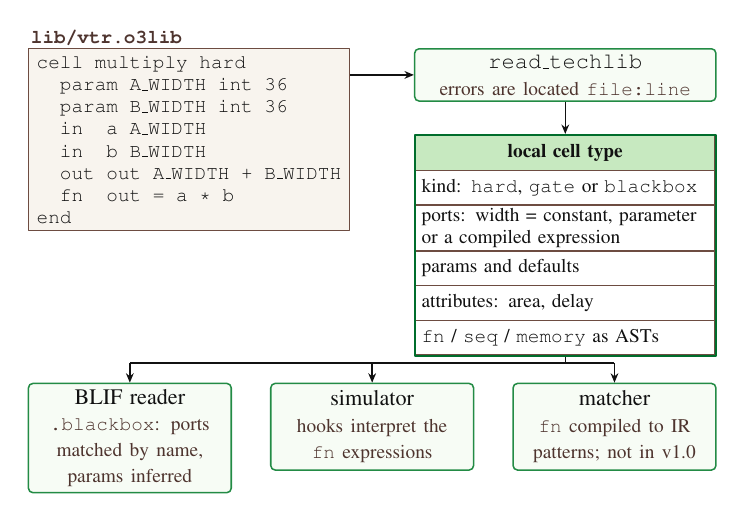
\begin{tikzpicture}[odin,
  fld/.style={draw=o3brn6, fill=white, line width=0.5pt, font=\scriptsize, align=left,
              text width=36.5mm, minimum height=4.4mm, inner xsep=2.2pt, inner ysep=1.2pt},
  use/.style={box, text width=24mm, minimum height=11mm}]
  % ---- source --------------------------------------------------------------------------------
  \node[draw=o3brn6, fill=o3brn1, line width=0.5pt, align=left, anchor=north west,
        inner xsep=3pt, inner ysep=2.5pt, font=\scriptsize\ttfamily,
        label={[font=\scriptsize\bfseries, color=o3brn7, anchor=south west, inner sep=1pt]
               north west:\odintt{lib/vtr.o3lib}}] (src) at (0, 0)
       {cell multiply hard\\
        \ \ param A\_WIDTH int 36\\
        \ \ param B\_WIDTH int 36\\
        \ \ in\ \ a A\_WIDTH\\
        \ \ in\ \ b B\_WIDTH\\
        \ \ out out A\_WIDTH + B\_WIDTH\\
        \ \ fn\ \ out = a * b\\
        end};
  % ---- reader and cell type ------------------------------------------------------------------
  \node[box, light, text width=36.5mm, anchor=north east] (rd) at (8.75, 0)
       {\odintt{read\_techlib}\\\odinsub{errors are located \odintt{file:line}}};
  \node[fld, fill=o3grn3, font=\scriptsize\bfseries, align=center, anchor=north]
       (h) at ($(rd.south)+(0,-0.42)$) {local cell type};
  \node[fld, anchor=north] (c1) at ($(h.south)+(0,\pgflinewidth)$) {kind: \odintt{hard}, \odintt{gate} or \odintt{blackbox}};
  \node[fld, anchor=north] (c2) at ($(c1.south)+(0,\pgflinewidth)$) {ports: width = constant, parameter or a compiled expression};
  \node[fld, anchor=north] (c3) at ($(c2.south)+(0,\pgflinewidth)$) {params and defaults};
  \node[fld, anchor=north] (c4) at ($(c3.south)+(0,\pgflinewidth)$) {attributes: area, delay};
  \node[fld, anchor=north] (c5) at ($(c4.south)+(0,\pgflinewidth)$) {\odintt{fn} / \odintt{seq} / \odintt{memory} as ASTs};
  \node[fit=(h)(c5), inner sep=0pt, draw=o3grn8, line width=0.7pt] (ct) {};
  % ---- users ---------------------------------------------------------------------------------
  \node[use, light, anchor=north west] (blif) at (0, -4.25)
       {BLIF reader\\\odinsub{\odintt{.blackbox}: ports matched by name, params inferred}};
  \node[use, light, anchor=north] (sim) at (4.375, -4.25)
       {simulator\\\odinsub{hooks interpret the \odintt{fn} expressions}};
  \node[use, light, anchor=north east] (pat) at (8.75, -4.25)
       {matcher\\\odinsub{\odintt{fn} compiled to IR patterns; not in v1.0}};
  % ---- edges ---------------------------------------------------------------------------------
  \draw[flow] (src.east |- rd) -- (rd.west);
  \draw[flow] (rd) -- (ct);
  \coordinate (rail) at ($(blif.north)+(0,0.25)$);
  \draw[line width=0.55pt, draw=o3ink] (ct.south) -- (ct.south |- rail);
  \draw[line width=0.55pt, draw=o3ink] (rail -| blif) -- (rail -| pat);
  \draw[flow] (rail -| blif) -- (blif.north);
  \draw[flow] (rail -| sim) -- (sim.north);
  \draw[flow] (rail -| pat) -- (pat.north);
\end{tikzpicture}
\end{odinfig}
\begin{odinfig}% The C ABI and plugin model (1D spec, DESIGN.md section 15.3, include/odin3/odin3.h ABI v4).
% Everything outside the core sees only odin3.h. Single column: \columnwidth.
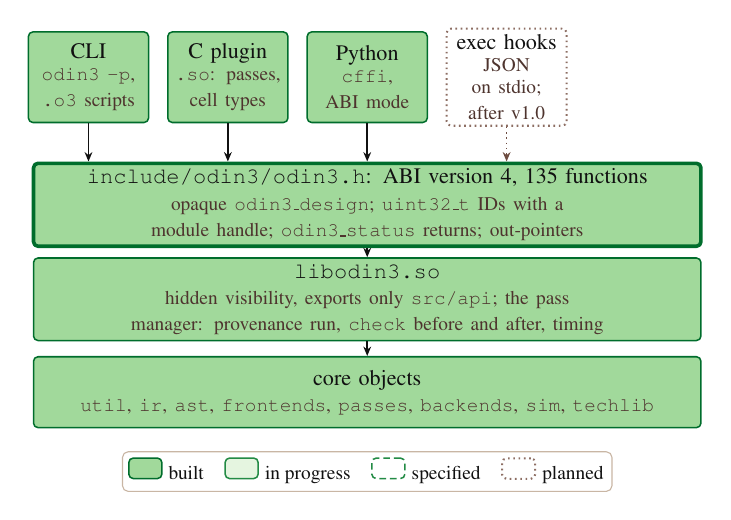
\begin{tikzpicture}[odin,
  client/.style={box, text width=14.2mm, minimum height=11.5mm, inner xsep=1.5pt},
  layer/.style={box, text width=83mm, minimum height=9mm}]
  % ---- clients -------------------------------------------------------------------------------
  \foreach \n/\x/\s/\t/\u in {
      cli/0.83/built/{CLI}/{\odintt{odin3 -p},\\\odintt{.o3} scripts},
      so/2.6/built/{C plugin}/{\odintt{.so}: passes,\\cell types},
      py/4.37/built/{Python}/{\odintt{cffi},\\ABI mode},
      hook/6.14/planned/{exec hooks}/{JSON on stdio;\\after v1.0}}
    \node[client, \s] (\n) at (\x, 0) {\t\\\odinsub{\u}};
  % ---- layers --------------------------------------------------------------------------------
  \node[layer, built, emph] (hdr) at (4.37, -1.62)
       {\odintt{include/odin3/odin3.h}: ABI version 4, 135 functions\\
        \odinsub{opaque \odintt{odin3\_design}; \odintt{uint32\_t} IDs with a module handle;
                 \odintt{odin3\_status} returns; out-pointers}};
  \node[layer, built] (lib) at (4.37, -2.82)
       {\odintt{libodin3.so}\\
        \odinsub{hidden visibility, exports only \odintt{src/api}; the pass manager: provenance
                 run, \odintt{check} before and after, timing}};
  \node[layer, built] (core) at (4.37, -4.0)
       {core objects\\
        \odinsub{\odintt{util}, \odintt{ir}, \odintt{ast}, \odintt{frontends}, \odintt{passes},
                 \odintt{backends}, \odintt{sim}, \odintt{techlib}}};
  % ---- edges ---------------------------------------------------------------------------------
  \foreach \n in {cli, so, py} \draw[flow] (\n.south) -- (\n.south |- hdr.north);
  \foreach \n in {hook}    \draw[flowplanned] (\n.south) -- (\n.south |- hdr.north);
  \draw[flow] (hdr) -- (lib);
  \draw[flow] (lib) -- (core);
  \odinlegend{anchor=north, at={(4.37, -4.75)}}
\end{tikzpicture}
\end{odinfig}
\end{document}
